% Generated for the Gini--Bayes paper
% Compile with XeLaTeX (run twice for references): xelatex gini-bayes.tex
\documentclass[12pt]{article}
\usepackage{fontspec}
\usepackage[protrusion=true]{microtype}
\usepackage{geometry}
\geometry{margin=1in}
\usepackage{graphicx}
\usepackage{amsmath}
\usepackage{booktabs}
\usepackage{siunitx}
\sisetup{table-format=1.4, table-number-alignment=center}
\usepackage[dvipsnames]{xcolor}
\usepackage{hyperref}
\usepackage{url}
\usepackage{setspace}
\usepackage[font=small,labelfont=bf,skip=6pt]{caption}
\usepackage{titlesec}
\titlespacing*{\section}{0pt}{1.2em}{0.6em}
\titlespacing*{\subsection}{0pt}{1em}{0.5em}
\titlespacing*{\subsubsection}{0pt}{0.9em}{0.4em}
\usepackage{enumitem}

% Code listings live in the GitHub repo (Appendix A); \texttt uses the default
% Latin Modern Mono, so no \setmonofont is needed (keeps the build TeX Live-only).

% --- figures: pgfplots (vector, native LaTeX; swap-friendly) ---
\usepackage{pgfplots}
\pgfplotsset{compat=1.18}
\usepgfplotslibrary{fillbetween}
\usetikzlibrary{patterns}
\definecolor{capblue}{HTML}{2C6FB5}
\definecolor{capred}{HTML}{C0392B}
\definecolor{capgray}{HTML}{7F8C8D}
\definecolor{capgreen}{HTML}{2E8B57}

% --- math font: match the Latin Modern text (load last, after amsmath/fontspec) ---
\usepackage{unicode-math}
\setmathfont{latinmodern-math.otf}

% No first-line indent; one consistent line of space between paragraphs
\setlength{\parindent}{0pt}
\setlength{\parskip}{0.6em}
\setlist{leftmargin=2em, itemsep=0.25em, topsep=0.5em, partopsep=0pt}
\setlength{\abovedisplayskip}{0.5em}
\setlength{\belowdisplayskip}{0.5em}
\setlength{\abovedisplayshortskip}{0.3em}
\setlength{\belowdisplayshortskip}{0.3em}

% shorthands
\newcommand{\pD}{p_D}
\newcommand{\PDx}{p(D \mid x)}
\newcommand{\slope}{\mathrm{slope}}
\newcommand{\AR}{\mathrm{AR}}
\newcommand{\WOE}{\mathrm{WOE}}
\newcommand{\IV}{\mathrm{IV}}
\newcommand{\E}{\mathbb{E}}

\begin{document}
\onehalfspacing

\title{The Gini--Bayes Connection:\\[0.3em]
\large The CAP Slope as Bayes' Theorem, with Applications to\\
Weight of Evidence, Somers' \emph{D}, and Calibration}
\author{Denis Burakov}
\date{June 2026}
\maketitle

\begin{abstract}
\noindent
The probabilistic reading of the cumulative accuracy profile (CAP) has a long industry
lineage. Falkenstein, Boral and Carty (2000) state, in discrete form, that the default
rate at a score percentile equals the portfolio average rate times the local slope of
the power curve; van der Burgt (2008, 2019) formalizes this as the continuous identity
$\PDx = \pD\, dy/dx$ and imports the continuous form as a working fact; Tasche (2009) analyzes the
resulting calibration method; Voloshyn and Voloshyn (2023) substitute Bayes' theorem,
$f(x\mid D)=\PDx f(x)/\pD$, into the area integral and write the Gini as a functional of the
calibration curve. Where Bayes enters this chain it does so under the area integral or band by
band (van der Burgt 2019); nowhere is the \emph{continuous} identity read differentially, as the
ratio of its two differentials --- which is exactly the CAP slope. We supply that differential
reading and three consequences. First, the
CAP slope is Bayes' theorem in cumulative coordinates, and the standardized PD it recovers
is the posterior rescaled by the prior. Second, the odds form of the same identity places
the weight of evidence, the Bayes factor, and the information value inside one geometry:
the weight of evidence at a point is the log of the ratio of the bad and good CAP slopes.
Third, we show that the accuracy ratio, Somers' $D_{yx}$, and the exact Gini
$(2A-1)/(1-\pD)$ are one number computed three ways, and that running the identity in
\emph{comparison mode} --- realized outcomes against model claims --- recovers the
reliability diagram in cumulative coordinates, with the gap between the empirical and
model-implied Ginis as its one-number summary. A worked five-band example carries every
identity, and a worked kernel-density example extends the construction to the continuous case,
recovering the weight-of-evidence and calibration curves from the class-conditional densities
alone.
\end{abstract}

\section{Introduction}

Discriminatory power and calibration are the two axes along which a credit rating system is
judged. Power asks whether the model orders borrowers correctly; calibration asks whether
the probabilities it attaches to them are right. The cumulative accuracy profile (CAP) and
its summary, the accuracy ratio (or Gini coefficient), are the standard instruments for the
first question, and a large industry literature treats them as power-only objects: the area
under the curve uses ranks and discards levels.

This separation is not as clean as it looks. The probabilistic reading of the CAP has an
industry lineage that quietly carries calibration inside a power object. Falkenstein, Boral
and Carty (2000), in the appendix of the Moody's RiskCalc methodology, state a discrete
relationship between the default-frequency curve and the power curve: the default rate at a
score percentile equals the portfolio mean rate times the local rise of the power curve.
Van der Burgt (2008) operationalizes this for low-default portfolios by fitting the CAP to a
one-parameter concave family and differentiating it to read off per-grade PDs; Tasche (2009)
analyzes that approach; van der Burgt (2019) writes the relationship as the continuous slope
identity
\begin{equation}\label{eq:slope-id}
\PDx \;=\; \pD\,\frac{dy}{dx},
\end{equation}
attributes it to Falkenstein et al.\ (2000), and uses the same geometry to construct the
rating scale itself. Voloshyn and Voloshyn (2023) substitute Bayes' theorem into the area
integral and obtain the Gini as a functional of the calibration curve.

In every step of this chain, \eqref{eq:slope-id} enters by citation rather than derivation.
It is never written that the slope identity is simply Bayes' theorem
\begin{equation}\label{eq:bayes-intro}
f(x\mid D)\;=\;\frac{\PDx\,f(x)}{\pD}
\end{equation}
differentiated in cumulative coordinates --- the ratio of the differential of the numerator
to the differential of $F(x)$. This paper supplies what the lineage assumes.

\paragraph{Contributions.} Our contribution is threefold.
\begin{enumerate}
\item \textbf{We derive the identity.} The CAP slope is Bayes' theorem in cumulative
coordinates (Section~\ref{sec:slope}), and the standardized PD it recovers,
$dF(x\mid D)/dF(x) = \PDx/\pD$, is the posterior rescaled by the prior.
\item \textbf{We extend it through the odds form.} The ratio of the bad and good CAP slopes
is the Bayes factor in favor of default, its logarithm is the weight of evidence, and the
Jeffreys divergence of the two slope profiles is the information value
(Section~\ref{sec:woe}). The standard scorecard quantities sit inside the same geometry.
\item \textbf{We run the identity in comparison mode.} Feeding it realized outcomes and
model claims produces an empirical and a model-implied CAP whose slope-by-slope agreement,
together with the level condition $\hat p_D = \pD$, is exactly calibration
(Section~\ref{sec:calib}): the reliability diagram in cumulative coordinates, with the gap
between the two Ginis as its one-number summary. Along the way we show that the accuracy
ratio, Somers' $D_{yx}$, and the exact Gini are the same number computed three ways
(Section~\ref{sec:somers}).
\end{enumerate}

We take the rating bands as given. Their construction is itself an application of this
geometry (van der Burgt 2019), and the regulatory requirement of a monotone PD scale is
precisely the concavity condition: slopes decreasing along the sort order. We treat the
discrete case throughout for clean derivations; Section~\ref{sec:continuous} gives the
continuous (density-estimation) reading.

One sentence summarizes the stance of the paper:
\begin{quote}
\emph{Slope $\times$ level $=$ PD is identity; the shape of the slope profile is assumption.}
\end{quote}
\begin{equation}
\underbrace{\text{PD}(x)}_{\PDx}
\;=\;
\underbrace{\langle D\rangle}_{\pD}
\,\cdot\,
\underbrace{\frac{dy}{dx}}_{\slope(x)},
\qquad \frac{dy}{dx}=\frac{dF(x\mid D)}{dF(x)}.
\end{equation}

\section{Setup and definitions}\label{sec:setup}

Borrowers carry an ordinal rating grade $x$, sorted from worst (riskiest) to best. The
default indicator is $Y\in\{0,1\}$, with $D=\{Y=1\}$. Three distributions organize
everything that follows:
\begin{itemize}
\item $f(x)$ --- the \textbf{marginal} (population) probability of grade $x$;
\item $\PDx$ --- the \textbf{posterior} conditional probability of default at grade $x$
(the calibration curve, in business terms the bad rate);
\item $f(x\mid D)$ --- the \textbf{likelihood}: the probability that a randomly chosen
defaulter carries grade $x$.
\end{itemize}
The unconditional (prior) default rate is the $f$-weighted average of the calibration curve,
\begin{equation}\label{eq:prior}
\pD \;=\; \int_0^1 \PDx\,f(x)\,dx
\qquad\text{(discretely, }\textstyle\pD=\sum_x \PDx f(x)\text{)}.
\end{equation}
Bayes' theorem ties the three together:
\begin{equation}\label{eq:bayes}
\underbrace{f(x\mid D)}_{\text{likelihood}}
=\frac{\overbrace{\PDx}^{\text{posterior}}\,\overbrace{f(x)}^{\text{marginal}}}
{\underbrace{\pD}_{\text{prior}}}.
\end{equation}
Read in words, $f(x\mid D)$ answers: \emph{if I pick a defaulter at random, what is the
probability they came from grade $x$?} A grade contributes more defaulters when its bad rate
$\PDx$ is high (it is risky) and when its population share $f(x)$ is large (many borrowers
sit there); the denominator $\pD$ normalizes the shares to sum to one.

\paragraph{Running example.} Table~\ref{tab:data} is the five-band portfolio we carry through
the paper. It has $N=115$ borrowers, $B=20$ defaulters, and prior $\pD = 20/115 = 0.1739$.

\begin{table}[htbp]
\centering
\small
\begin{tabular}{l S[table-format=3.0] S[table-format=2.0] S[table-format=2.0]
  S[table-format=1.4] S[table-format=1.4] S[table-format=1.4] S[table-format=1.4]}
\toprule
Band & {Count} & {Goods} & {Bads} & {$\PDx$} & {$f(x)$} & {$f(x\mid D)$} & {$f(x\mid\bar D)$}\\
\midrule
A & 24 & 23 & 1 & 0.0417 & 0.2087 & 0.0500 & 0.2421 \\
B & 36 & 32 & 4 & 0.1111 & 0.3130 & 0.2000 & 0.3368 \\
C & 25 & 20 & 5 & 0.2000 & 0.2174 & 0.2500 & 0.2105 \\
D & 20 & 15 & 5 & 0.2500 & 0.1739 & 0.2500 & 0.1579 \\
E & 10 &  5 & 5 & 0.5000 & 0.0870 & 0.2500 & 0.0526 \\
\midrule
Total & 115 & 95 & 20 & & & & \\
\bottomrule
\end{tabular}
\caption{The five-band running example. $f(x)=\text{count}/115$, $f(x\mid D)=\text{bads}/20$,
$f(x\mid\bar D)=\text{goods}/95$. Prior $\pD=0.1739$.}
\label{tab:data}
\end{table}

A one-line check of Bayes \eqref{eq:bayes} on band E (writing $x{=}E$ for the rating):
\begin{equation}
f(x{=}E\mid D)=\frac{p(D\mid x{=}E)\,f(x{=}E)}{\pD}
=\frac{0.50\times \tfrac{10}{115}}{\tfrac{20}{115}}
=0.50\times\frac{10}{20}=0.25,
\end{equation}
matching $5$ defaulters out of $20$. Band E has the highest bad rate ($50\%$) but the
smallest population share; band B has a low bad rate ($11\%$) but the largest share. Bayes
balances the two into the defaulter mix $f(x\mid D)$. Figure~\ref{fig:bars} shows the inputs
and the Bayes reweighting side by side.

\begin{figure}[htbp]
\centering
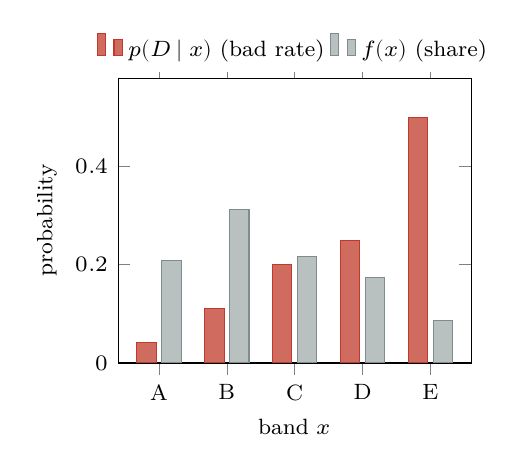
\begin{tikzpicture}
\begin{axis}[
  width=0.5\textwidth, height=5.2cm,
  ybar, bar width=7pt,
  ymin=0, ymax=0.58,
  symbolic x coords={A,B,C,D,E}, xtick=data,
  ylabel={probability}, xlabel={band $x$},
  legend style={at={(0.5,1.02)},anchor=south,draw=none,legend columns=2,font=\footnotesize},
  tick label style={font=\footnotesize}, label style={font=\footnotesize},
  enlarge x limits=0.15,
]
\addplot[fill=capred!75,draw=capred] coordinates {(A,0.0417)(B,0.1111)(C,0.2000)(D,0.2500)(E,0.5000)};
\addplot[fill=capgray!55,draw=capgray] coordinates {(A,0.2087)(B,0.3130)(C,0.2174)(D,0.1739)(E,0.0870)};
\legend{$\PDx$ (bad rate),$f(x)$ (share)}
\end{axis}
\end{tikzpicture}\hfill
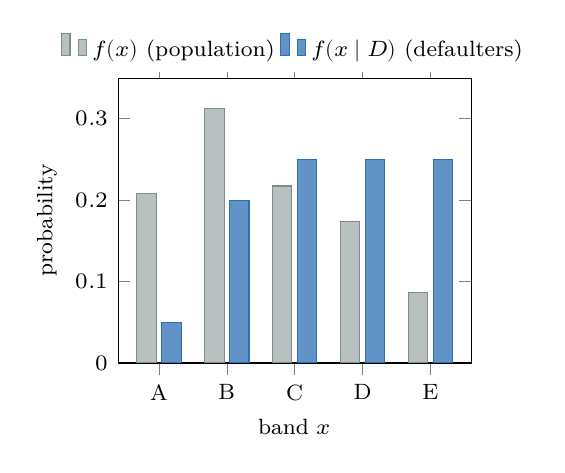
\begin{tikzpicture}
\begin{axis}[
  width=0.5\textwidth, height=5.2cm,
  ybar, bar width=7pt,
  ymin=0, ymax=0.35,
  symbolic x coords={A,B,C,D,E}, xtick=data,
  ylabel={probability}, xlabel={band $x$},
  legend style={at={(0.5,1.02)},anchor=south,draw=none,legend columns=2,font=\footnotesize},
  tick label style={font=\footnotesize}, label style={font=\footnotesize},
  enlarge x limits=0.15,
]
\addplot[fill=capgray!55,draw=capgray] coordinates {(A,0.2087)(B,0.3130)(C,0.2174)(D,0.1739)(E,0.0870)};
\addplot[fill=capblue!75,draw=capblue] coordinates {(A,0.0500)(B,0.2000)(C,0.2500)(D,0.2500)(E,0.2500)};
\legend{$f(x)$ (population),$f(x\mid D)$ (defaulters)}
\end{axis}
\end{tikzpicture}
\caption{\textbf{Left:} the two ingredients of Bayes --- the calibration curve $\PDx$ and the
population share $f(x)$. \textbf{Right:} Bayes reweights the population $f(x)$ (grey) into the
defaulter mix $f(x\mid D)$ (blue), pulling mass toward the riskier bands. Grey exceeds blue in
the safe bands A--B, where defaulters are under-represented relative to the population, and blue
exceeds grey in the risky bands C--E, where they are over-represented; the crossover is the
reweighting by the bad rate $\PDx$. The denominator $\pD$ normalizes $f(x\mid D)$ to sum to one.}
\label{fig:bars}
\end{figure}

\section{The CAP slope is Bayes' theorem}\label{sec:slope}

The CAP curve plots the cumulative share of defaulters captured, $F(x\mid D)$, against the
cumulative share of population, $F(x)$, both sorted worst-first:
\begin{equation}
F(x\mid D)=\int_{\text{worst}}^{x} f(t\mid D)\,dt,
\qquad
F(x)=\int_{\text{worst}}^{x} f(t)\,dt .
\end{equation}
Its integrand is the defaulter density $f(x\mid D)$, which Bayes \eqref{eq:bayes} expresses
through the calibration curve. The \emph{slope} of the CAP at an operating point is the
derivative of one cumulative against the other, and by the chain rule it is the ratio of the
two integrands:
\begin{equation}\label{eq:cap-slope}
\boxed{\;
\frac{dF(x\mid D)}{dF(x)}
=\frac{f(x\mid D)}{f(x)}
=\frac{\PDx}{\pD}
\;}
\end{equation}
where the last step is exactly Bayes' theorem \eqref{eq:bayes} with the common factor $f(x)$
cancelled. Multiplying back by the prior recovers the calibration curve,
\begin{equation}\label{eq:pd-from-slope}
\PDx \;=\; \pD\cdot\frac{dF(x\mid D)}{dF(x)},
\end{equation}
which is the slope identity \eqref{eq:slope-id}. The derivation is one line: the CAP slope is
Bayes' theorem in cumulative coordinates, and the quantity it returns,
\begin{equation}
\mathrm{PD}_{\text{st}}(x)\;:=\;\frac{\PDx}{\pD}\;=\;\frac{dF(x\mid D)}{dF(x)},
\end{equation}
is the \textbf{standardized PD} --- the posterior rescaled by the prior, i.e.\ how many times
the portfolio-average risk a borrower at grade $x$ carries.

\paragraph{Provenance.} Equation~\eqref{eq:pd-from-slope} appears in Falkenstein et al.\ (2000,
App.~4A) in discrete, verbal form: with $\mathrm{prob}(q)$ the default frequency at
percentile $q$ and $\mathrm{power}(q)$ the power-curve height,
$\mathrm{prob}(q)=100\cdot\overline{\mathrm{prob}}\cdot\big(\mathrm{power}(q)-\mathrm{power}(q-1)\big)$,
i.e.\ PD $=$ mean-PD $\times$ discrete CAP slope (the $1/100$ is the percentile step). They
neither write it as a derivative nor invoke Bayes. Van der Burgt (2019, Eq.~2.3) gives the
continuous form $\PDx=\pD\,[dy/dx]$ and the per-grade version
$P_r=\frac{y_r-y_{r-1}}{x_r-x_{r-1}}\pD$, deriving the latter from Bayes' law applied to a
single band. What \eqref{eq:cap-slope} adds is the observation that the \emph{continuous}
identity is itself nothing but Bayes \eqref{eq:bayes} differentiated --- the ratio of
$dF(x\mid D)=f(x\mid D)\,dx$ to $dF(x)=f(x)\,dx$ --- so the per-band Bayes step and the
slope identity are the same statement at two resolutions.

\paragraph{The CAP of the running example.} Accumulating Table~\ref{tab:data} worst-first
(E, D, C, B, A) gives the curve in Figure~\ref{fig:cap}.

\begin{table}[htbp]
\centering
\small
\begin{tabular}{l S[table-format=1.4] S[table-format=1.4] S[table-format=1.4] S[table-format=1.4]}
\toprule
Sorted (worst first) & {$f(x)$} & {$F(x)$} & {$f(x\mid D)$} & {$F(x\mid D)$}\\
\midrule
E & 0.0870 & 0.0870 & 0.2500 & 0.2500 \\
D & 0.1739 & 0.2609 & 0.2500 & 0.5000 \\
C & 0.2174 & 0.4783 & 0.2500 & 0.7500 \\
B & 0.3130 & 0.7913 & 0.2000 & 0.9500 \\
A & 0.2087 & 1.0000 & 0.0500 & 1.0000 \\
\bottomrule
\end{tabular}
\caption{Cumulative coordinates of the CAP curve, sorted worst-first.}
\label{tab:cap}
\end{table}

\begin{figure}[htbp]
\centering
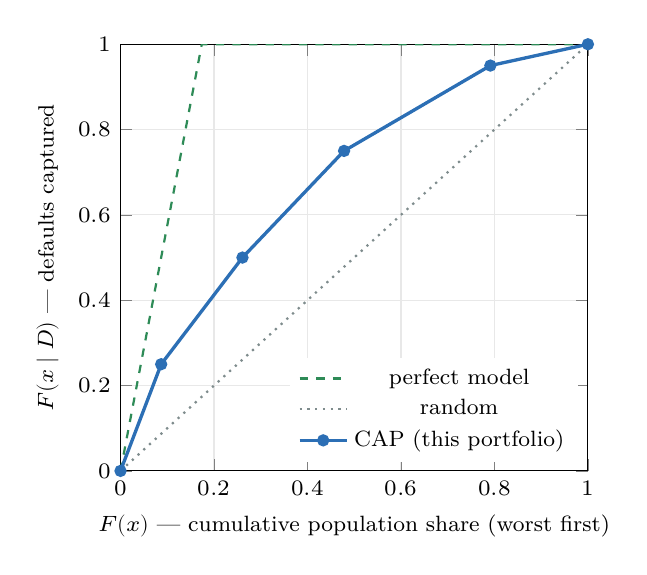
\begin{tikzpicture}
\begin{axis}[
  width=0.62\textwidth, height=7cm,
  xmin=0,xmax=1,ymin=0,ymax=1,
  xlabel={$F(x)$ --- cumulative population share (worst first)},
  ylabel={$F(x\mid D)$ --- defaults captured},
  legend style={at={(0.98,0.02)},anchor=south east,draw=none,font=\footnotesize},
  tick label style={font=\footnotesize}, label style={font=\footnotesize},
  grid=major, grid style={gray!18},
]
% perfect model boundary through (p_D,1)
\addplot[capgreen,dashed,thick] coordinates {(0,0)(0.1739,1)(1,1)};
\addlegendentry{perfect model}
% random diagonal
\addplot[capgray,dotted,thick] coordinates {(0,0)(1,1)};
\addlegendentry{random}
% empirical CAP
\addplot[capblue,very thick,mark=*,mark size=1.6pt]
  coordinates {(0,0)(0.0870,0.25)(0.2609,0.50)(0.4783,0.75)(0.7913,0.95)(1,1)};
\addlegendentry{CAP (this portfolio)}
\end{axis}
\end{tikzpicture}
\caption{The CAP curve of Table~\ref{tab:cap}. The slope of each segment is the standardized PD
of that band; multiplied by $\pD$ it returns the band's bad rate
(Eq.~\ref{eq:pd-from-slope}). The perfect-model boundary reaches $(\pD,1)=(0.1739,1)$, not
$(0,1)$ --- the fact behind the $1-\pD$ correction in Section~\ref{sec:somers}.}
\label{fig:cap}
\end{figure}

\section{The odds form: weight of evidence, Bayes factor, information value}\label{sec:woe}

Everything above used the ``bad'' CAP. The complementary ``good'' CAP accumulates the survivor
density $f(x\mid\bar D)$, and its slope is the standardized survival rate:
\begin{equation}
\frac{dF(x\mid D)}{dF(x)}=\frac{\PDx}{\pD},
\qquad
\frac{dF(x\mid\bar D)}{dF(x)}=\frac{1-\PDx}{1-\pD}.
\end{equation}
The two slopes are not independent: since $f(x)=\pD f(x\mid D)+(1-\pD)f(x\mid\bar D)$, they
satisfy the mixture identity $\pD\,\slope_{\text{bad}}(x)+(1-\pD)\,\slope_{\text{good}}(x)=1$ at
every point, so the bad CAP rises above the diagonal exactly where the good CAP dips below.

Bayes' theorem in odds form states posterior odds $=$ likelihood ratio $\times$ prior odds.
Dividing the two slopes is exactly that statement, with $f(x)$ cancelling:
\begin{equation}\label{eq:woe}
\underbrace{\frac{\PDx/\pD}{(1-\PDx)/(1-\pD)}}_{\text{ratio of CAP slopes}}
=\underbrace{\frac{\PDx}{1-\PDx}}_{\text{posterior odds}}\cdot
\underbrace{\frac{1-\pD}{\pD}}_{1/\text{prior odds}}
=\frac{f(x\mid D)}{f(x\mid\bar D)}
=e^{\WOE(x)} .
\end{equation}
The middle quantity is the \textbf{Bayes factor} in favor of default, $\mathrm{BF}(x)$, and its
logarithm is the \textbf{weight of evidence}:
\begin{equation}\label{eq:woe-def}
\boxed{\;\WOE(x)=\ln\frac{\slope_{\text{bad}}(x)}{\slope_{\text{good}}(x)}
=\ln\frac{f(x\mid D)}{f(x\mid\bar D)}\;}
\end{equation}
(bad-over-good convention; the industry good-over-bad convention flips the sign). The weight
of evidence at a point is the log of the ratio of the two CAP slopes.

\paragraph{Verification on band E.} The bad slope is $0.25/0.087=2.875$ and the good slope is
$0.5/0.826=0.605$, a ratio of $4.75$. Directly,
$f(E\mid D)/f(E\mid\bar D)=0.25/(5/95)=4.75$, so $\WOE(E)=\ln 4.75=1.558$.

\paragraph{Information value.} The slope table is one step from the information value. Weighting
each band's evidence by the gap between the two likelihoods gives
\begin{equation}\label{eq:iv}
\IV=\sum_x \bigl(f(x\mid D)-f(x\mid\bar D)\bigr)\,\WOE(x),
\end{equation}
the Jeffreys (symmetrized Kullback--Leibler) divergence between the defaulter and survivor
score distributions. Every term is nonnegative because the difference and the log-likelihood
ratio always share a sign (Table~\ref{tab:iv}).

\begin{table}[htbp]
\centering
\small
\begin{tabular}{l S[table-format=1.3] S[table-format=1.3]
  S[table-format=-1.3] S[table-format=-1.3] S[table-format=1.3]}
\toprule
Band & {$f(x\mid D)$} & {$f(x\mid\bar D)$} & {Difference} & {$\WOE(x)$} & {Contribution}\\
\midrule
A & 0.050 & 0.242 & -0.192 & -1.577 & 0.303 \\
B & 0.200 & 0.337 & -0.137 & -0.521 & 0.071 \\
C & 0.250 & 0.211 &  0.039 &  0.172 & 0.007 \\
D & 0.250 & 0.158 &  0.092 &  0.460 & 0.042 \\
E & 0.250 & 0.053 &  0.197 &  1.558 & 0.308 \\
\midrule
Total & & & & & 0.731 \\
\bottomrule
\end{tabular}
\caption{Information value of the running example, $\IV=0.731$. The weight of evidence in the
fifth column is $\ln(\slope_{\text{bad}}/\slope_{\text{good}})$ by Eq.~\eqref{eq:woe-def}.}
\label{tab:iv}
\end{table}

The scorecard trio --- standardized PD, weight of evidence, information value --- thus lives
entirely inside CAP geometry: the standardized PD is one slope, the weight of evidence is the
log-ratio of two slopes, and the information value is the divergence between the two slope
profiles. This recovers, from the CAP side, the information-theoretic framework of Sudjianto
and Burakov (2025); the weight-of-evidence reading as a Bayes-factor explanation follows
Alvarez-Melis (2019, 2021).

\section{Accuracy ratio, Somers' \texorpdfstring{$D$}{D}, and the exact Gini}\label{sec:somers}

The area under the CAP, $A=\int_0^1 F(x\mid D)\,dF(x)$, summarizes power in one number. For
the running example the trapezoidal area is $A=0.6815$. A common shortcut reports
$\AR\approx 2A-1=0.363$, but this is valid only when $\pD\approx 0$. The exact accuracy ratio
carries a $1-\pD$ correction,
\begin{equation}\label{eq:ar-exact}
\AR=\frac{2A-1}{1-\pD}=\frac{2(0.6815)-1}{1-0.1739}=\frac{0.363}{0.826}=0.4395,
\end{equation}
because the perfect-model boundary in CAP coordinates reaches $(\pD,1)$, not $(0,1)$
(Figure~\ref{fig:cap}): the maximum attainable area is $1-\pD/2$, not $1$. Van der Burgt
(2019, Eq.~2.6) and Voloshyn and Voloshyn (2023, Eq.~1, after Thomas 2009) both use the exact
form; van der Burgt (2008) uses the approximation $\AR\approx 2A-1$.

\paragraph{Somers' $D$ via pair counting.} The same $0.4395$ arises with no curve at all, by
counting concordant and discordant good--bad pairs. Take one good and one bad borrower; the
pair is \emph{concordant} if the bad sits in a riskier band than the good, \emph{discordant}
if the good sits in a riskier band, and \emph{tied} if they share a band. Somers'
$D_{yx}$ --- the rank correlation of the default outcome $y$ with the rating $x$ --- is
\begin{equation}\label{eq:somers}
D_{yx}=\frac{P-Q}{n_{\text{good}}\,n_{\text{bad}}},
\end{equation}
with $P$ concordant and $Q$ discordant pairs (the Kendall convention; the symbol $D$ is reserved
for the default event) and all $n_{\text{good}}n_{\text{bad}}$ good--bad pairs (including ties) in
the denominator. These pairs are drawn from the rating-by-outcome contingency table
(Table~\ref{tab:contingency}); Table~\ref{tab:pairs} carries out the count:
$P=1192$, $Q=357$, ties $=351$, total $=95\times20=1900$, so
\begin{equation}
D_{yx}=\frac{1192-357}{1900}=0.4395 .
\end{equation}

\begin{table}[htbp]
\centering
\small
\begin{tabular}{l r r r}
\toprule
Rating $x$ & Goods & Bads & Total \\
\midrule
A & 23 & 1 & 24 \\
B & 32 & 4 & 36 \\
C & 20 & 5 & 25 \\
D & 15 & 5 & 20 \\
E & 5 & 5 & 10 \\
\midrule
Total & 95 & 20 & 115 \\
\bottomrule
\end{tabular}
\caption{The rating-by-outcome contingency table. Pairing each of the $95$ goods with each of
the $20$ bads gives $n_{\text{good}}n_{\text{bad}}=1900$ good--bad pairs; classifying each as
concordant, discordant, or tied by rating (Table~\ref{tab:pairs}) yields Somers' $D_{yx}$.}
\label{tab:contingency}
\end{table}

\begin{table}[htbp]
\centering
\small
\begin{tabular}{l r r}
\toprule
Band of the good & Concordant (bad riskier) & Discordant (good riskier)\\
\midrule
A (23 goods) & $23\times(4{+}5{+}5{+}5)=437$ & $23\times 0 = 0$ \\
B (32 goods) & $32\times(5{+}5{+}5)=480$ & $32\times 1 = 32$ \\
C (20 goods) & $20\times(5{+}5)=200$ & $20\times(4{+}1)=100$ \\
D (15 goods) & $15\times 5 = 75$ & $15\times(5{+}4{+}1)=150$ \\
E (5 goods)  & $5\times 0 = 0$ & $5\times(5{+}5{+}4{+}1)=75$ \\
\midrule
Total & $1192$ & $357$ \\
\bottomrule
\end{tabular}
\caption{Concordant/discordant good--bad pair counts. ``Bad riskier'' counts, for the goods in
a band, all bads in riskier bands; ``good riskier'' counts all bads in safer bands. Ties (same
band) are $1900-1192-357=351$.}
\label{tab:pairs}
\end{table}

\paragraph{One number, three routes.} The accuracy ratio, Somers' $D_{yx}$, and the
Mann--Whitney form of the ROC Gini coincide exactly:
\begin{equation}\label{eq:three-routes}
\AR=\underbrace{\frac{2A-1}{1-\pD}}_{\text{CAP area}}
=\underbrace{\frac{P-Q}{n_{\text{good}}n_{\text{bad}}}}_{\text{Somers' }D_{yx}}
=\underbrace{2\,\mathrm{AUC}-1}_{\text{ROC}}
=0.4395,
\qquad
\mathrm{AUC}=\frac{P+\tfrac12 T}{n_{\text{good}}n_{\text{bad}}}=0.7197 .
\end{equation}
The CAP route integrates the curve and corrects by $1-\pD$; the pair-counting route never
draws a curve; the ROC route counts the same pairs with ties split. All three are the same
rank statistic, and the $1-\pD$ in \eqref{eq:ar-exact} is precisely what reconciles the
curve-area route with the pair-counting route. The approximation $2A-1=0.363$ fails the
identity; the exact form passes it.

\section{Calibration in cumulative coordinates}\label{sec:calib}

So far the calibration curve $\PDx$ has been the observed bad rate, and the CAP has recovered
it through \eqref{eq:pd-from-slope}. But \eqref{eq:cap-slope}--\eqref{eq:pd-from-slope} hold
for \emph{any} function placed in the $\PDx$ slot, provided $\pD$ is its own $f$-weighted
average. Whether that function coincides with observed default frequencies is a separate
question --- and that question is calibration. Running the identity in comparison mode turns
it into a calibration diagnostic.

\paragraph{Two CAPs.} Sort all borrowers worst-first by the model's score and accumulate two
quantities.
\begin{itemize}
\item \textbf{Empirical CAP} (the outcome): accumulate realized defaults $y_i\in\{0,1\}$,
\begin{equation}
F_{\text{emp}}(x\mid D)=\frac{\sum_{i\le x}y_i}{\sum_i y_i}.
\end{equation}
Its slope, rescaled by the realized level, recovers the observed frequencies:
$\slope_{\text{emp}}(x)\cdot\pD=\E[Y\mid x]$.
\item \textbf{Model-implied CAP} (the promise): accumulate the claimed probabilities $\hat p_i$,
treating each borrower as $\hat p_i$ expected defaults,
\begin{equation}
F_{\text{model}}(x\mid D)=\frac{\sum_{i\le x}\hat p_i}{\sum_i \hat p_i}.
\end{equation}
Its slope recovers the claims: $\slope_{\text{model}}(x)\cdot\hat p_D=\hat p(D\mid x)$, where
$\hat p_D=\sum_x f(x)\,\hat p(D\mid x)$ is the model's average claim.
\end{itemize}
The model-implied CAP is the model's forecast of its own CAP --- the curve that would
materialize if the claimed PDs were the truth.

\paragraph{Calibration as coincidence of the two curves.} Perfect calibration is the statement
that the two CAPs agree everywhere, which splits into a shape condition and a level condition:
\begin{equation}\label{eq:calib-cond}
\hat p(D\mid x)=\E[Y\mid x]\ \ \forall x
\;\;\Longleftrightarrow\;\;
\hat p_D=\pD
\ \text{ and }\
\slope_{\text{model}}(x)=\slope_{\text{emp}}(x)\ \ \forall x .
\end{equation}
Differentiating each curve band by band and rescaling by its own level maps the picture into
reliability-diagram coordinates:
\begin{equation}\label{eq:reliability}
\bigl(\hat p(D\mid x),\,\E[Y\mid x]\bigr)
=\bigl(\slope_{\text{model}}(x)\cdot\hat p_D,\ \slope_{\text{emp}}(x)\cdot\pD\bigr),
\end{equation}
a point on the reliability diagram; perfect calibration places every band on the $45^\circ$
line. The two views carry identical information: the reliability diagram is the derivative of
the CAP comparison, and the CAP comparison is the cumulative integral of the reliability
diagram. The gap between the empirical and model-implied Ginis is the one-number summary, with
the caveat that pointwise deviations can cancel in the area, so
the band-level comparison remains the fundamental object. The calibration reference in CAP
coordinates is the \emph{empirical} curve itself --- it plays the role of the $45^\circ$
diagonal in the reliability diagram --- not the perfect-model boundary through $(\pD,1)$,
which is a ranking ideal irrelevant to calibration.

\paragraph{Comparison on the running example.} Suppose a model ranks the five bands correctly
but compresses risk in log-odds, $\operatorname{logit}\hat p(D\mid x)=\alpha+\beta\,
\operatorname{logit}p(D\mid x)$ with $(\alpha,\beta)=(-0.4,0.6)$ --- the standard
recalibration form, linear in log-odds, going back to Cox (1958). The claimed PDs and the
resulting model-implied CAP are in
Table~\ref{tab:calib}; the two CAPs and the reliability diagram are in
Figure~\ref{fig:calib}. The level is nearly right ($\hat p_D=0.199$ vs.\ $\pD=0.174$) but the
shape is flattened, and the model-implied Gini collapses to $0.282$ against the empirical
$0.4395$. The sign of the gap is diagnostic: model-implied \emph{below} empirical means the
claims are less dispersed than the outcomes --- a recalibration slope above one (the forward
compression $\beta=0.6$ inverts to a Cox slope $\approx 1.67$) --- while the reverse ordering,
model-implied above empirical, is the overconfidence signature. This level-versus-shape split is
the cumulative-coordinate counterpart of the calibration-curve factor decomposition of Voloshyn
and Voloshyn (2023), whose curve is linear in PD ($p(D\mid x)=ax+b$) rather than log-odds.

\begin{table}[htbp]
\centering
\small
\begin{tabular}{l S[table-format=1.4] S[table-format=1.4] S[table-format=1.4] S[table-format=1.4]}
\toprule
Sorted worst-first & {$\hat p(D\mid x)$} & {$\E[Y\mid x]$} & {$F_{\text{model}}(x\mid D)$} & {$F_{\text{emp}}(x\mid D)$}\\
\midrule
E & 0.4013 & 0.5000 & 0.1757 & 0.2500 \\
D & 0.2575 & 0.2500 & 0.4011 & 0.5000 \\
C & 0.2259 & 0.2000 & 0.6483 & 0.7500 \\
B & 0.1614 & 0.1111 & 0.9026 & 0.9500 \\
A & 0.0927 & 0.0500 & 1.0000 & 1.0000 \\
\midrule
\multicolumn{3}{l}{Gini (empirical $=0.4395$, model $=0.2823$)} & & \\
\bottomrule
\end{tabular}
\caption{Comparison mode on the running example. The model preserves the ranking but
compresses the slope profile; the gap between the empirical and model-implied CAPs is the
calibration error.}
\label{tab:calib}
\end{table}

\begin{figure}[htbp]
\centering
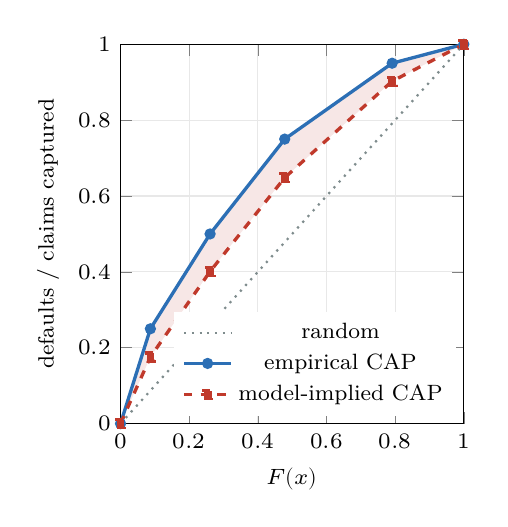
\begin{tikzpicture}
\begin{axis}[
  width=0.49\textwidth,height=6.4cm,
  xmin=0,xmax=1,ymin=0,ymax=1,
  xlabel={$F(x)$}, ylabel={defaults / claims captured},
  legend style={at={(0.98,0.02)},anchor=south east,draw=none,font=\footnotesize},
  tick label style={font=\footnotesize}, label style={font=\footnotesize},
  grid=major, grid style={gray!18},
]
\addplot[capgray,dotted,thick] coordinates {(0,0)(1,1)};
\addplot[capblue,very thick,mark=*,mark size=1.4pt,name path=emp]
  coordinates {(0,0)(0.0870,0.25)(0.2609,0.50)(0.4783,0.75)(0.7913,0.95)(1,1)};
\addplot[capred,very thick,dashed,mark=square*,mark size=1.4pt,name path=mod]
  coordinates {(0,0)(0.0870,0.1757)(0.2609,0.4011)(0.4783,0.6483)(0.7913,0.9026)(1,1)};
\addplot[capred!12] fill between[of=emp and mod];
\legend{random,empirical CAP,model-implied CAP}
\end{axis}
\end{tikzpicture}\hfill
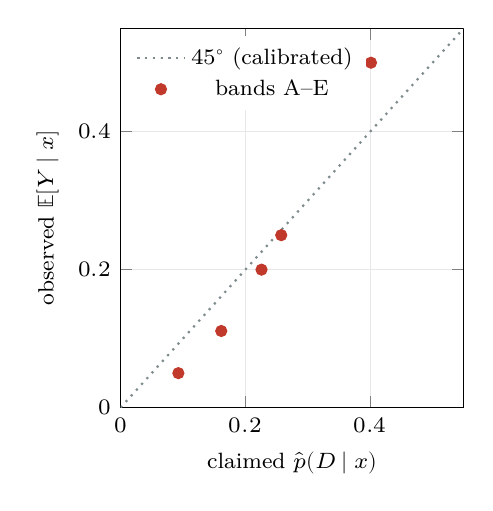
\begin{tikzpicture}
\begin{axis}[
  width=0.49\textwidth,height=6.4cm,
  xmin=0,xmax=0.55,ymin=0,ymax=0.55,
  xlabel={claimed $\hat p(D\mid x)$}, ylabel={observed $\E[Y\mid x]$},
  legend style={at={(0.02,0.98)},anchor=north west,draw=none,font=\footnotesize},
  tick label style={font=\footnotesize}, label style={font=\footnotesize},
  grid=major, grid style={gray!18},
]
\addplot[capgray,dotted,thick] coordinates {(0,0)(0.55,0.55)};
\addplot[only marks,capred,mark=*,mark size=2pt]
  coordinates {(0.0927,0.05)(0.1614,0.1111)(0.2259,0.20)(0.2575,0.25)(0.4013,0.50)};
\legend{$45^\circ$ (calibrated),bands A--E}
\end{axis}
\end{tikzpicture}
\caption{\textbf{Left:} empirical vs.\ model-implied CAP; the shaded area is the shape part of
the calibration error. \textbf{Right:} the same information as a reliability diagram --- the
band-by-band derivative of the left panel, rescaled by each level
(Eq.~\ref{eq:reliability}). Band E sits \emph{above} the $45^\circ$ line --- the model
under-predicts the riskiest band --- while bands A--D sit below it, over-predicting: the
compressed slope profile is too timid at both ends.}
\label{fig:calib}
\end{figure}

\paragraph{Two models, one Gini.} The diagnostic earns its keep when two models rank borrowers
identically but disagree on the probabilities --- a difference the Gini cannot see.
Figure~\ref{fig:twomodels} puts two such models on one portfolio: their scores are monotone
transforms of each other, so they share a single empirical CAP and a single Gini ($0.59$).
Model~A claims the realized PDs; Model~B is overconfident, pushing its claims too far in
log-odds. The area cannot separate them --- the empirical curve is the same for both --- yet
their model-implied curves diverge: A's claimed Gini ($0.58$) matches the empirical, while B's
($0.78$) overstates its own discrimination, and B's reliability points bow off the $45^\circ$
line. The gap between each model's implied Gini and the empirical Gini is the calibration
summary; the Gini alone is blind to it.

\begin{figure}[htbp]
\centering
\begin{tikzpicture}
\begin{axis}[
  width=0.49\textwidth,height=6.4cm, xmin=0,xmax=1,ymin=0,ymax=1.02,
  xlabel={$F(x)$ (worst first)}, ylabel={$F(x\mid D)$},
  tick label style={font=\footnotesize}, label style={font=\footnotesize},
  grid=major, grid style={gray!15},
  legend style={at={(0.97,0.03)},anchor=south east,draw=none,font=\scriptsize},
]
\addplot[capgray,dotted,thick] coordinates {(0,0)(1,1)}; \addlegendentry{random}
\addplot[black,very thick] table[x=Fx,y=Femp]{data/compare_cap.dat}; \addlegendentry{empirical}
\addplot[capblue,very thick,dashed] table[x=Fx,y=FmodA]{data/compare_cap.dat}; \addlegendentry{Model A claims}
\addplot[capred,very thick,dashed] table[x=Fx,y=FmodB]{data/compare_cap.dat}; \addlegendentry{Model B claims}
\node[font=\scriptsize,anchor=north west,align=left] at (axis cs:0.05,0.99)
 {Gini $=0.59$ (both)\\[1pt]\textcolor{capblue}{A claims $0.58$}\\\textcolor{capred}{B claims $0.78$}};
\end{axis}
\end{tikzpicture}\hfill
\begin{tikzpicture}
\begin{axis}[
  width=0.49\textwidth,height=6.4cm, xmin=0,xmax=0.85,ymin=0,ymax=0.85,
  xlabel={predicted $\hat p(D\mid x)$}, ylabel={observed $\E[Y\mid x]$},
  tick label style={font=\footnotesize}, label style={font=\footnotesize},
  grid=major, grid style={gray!15},
  legend style={at={(0.03,0.97)},anchor=north west,draw=none,font=\scriptsize},
]
\addplot[capgray,dotted,thick] coordinates {(0,0)(0.85,0.85)}; \addlegendentry{calibrated}
\addplot[capblue,thick,mark=*,mark size=1.4pt] table[x=pA,y=EA]{data/compare_rel.dat}; \addlegendentry{Model A}
\addplot[capred,thick,mark=square*,mark size=1.4pt] table[x=pB,y=EB]{data/compare_rel.dat}; \addlegendentry{Model B (overconfident)}
\end{axis}
\end{tikzpicture}
\caption{Two models with identical ranking, hence identical empirical Gini (left), but different
calibration (right). Both share the empirical CAP; Model~A's claimed CAP sits on it (claimed
Gini $0.58$ vs.\ empirical $0.59$), while the overconfident Model~B's claimed CAP overstates
discrimination (claimed Gini $0.78$) and its reliability points bow off the $45^\circ$ line ---
a gap the area-based Gini cannot see.}
\label{fig:twomodels}
\end{figure}

\section{The continuous case: density estimation}\label{sec:continuous}

The discrete derivation transfers verbatim to continuous scores once the three distributions
are estimated as densities rather than band frequencies. The CAP slope \eqref{eq:cap-slope} is
a ratio of densities,
\begin{equation}
\frac{dF(x\mid D)}{dF(x)}=\frac{f(x\mid D)}{f(x)}=\frac{\PDx}{\pD},
\end{equation}
and the weight of evidence \eqref{eq:woe-def} is a log-ratio of class-conditional densities,
$\WOE(x)=\ln f(x\mid D)-\ln f(x\mid\bar D)$. Both reduce to estimating the class-conditional
densities $f(x\mid D)$ and $f(x\mid\bar D)$. Alvarez-Melis (2019, 2021) does exactly this for
weight-of-evidence explanations: fit a kernel density estimator (or a Gaussian model) to each
class and take the log-density difference,
\begin{equation}
\hat f(x\mid c)=\frac{1}{n_c}\sum_{i:\,y_i=c}K_h(x-x_i),
\qquad
\widehat{\WOE}(x)=\ln\hat f(x\mid D)-\ln\hat f(x\mid\bar D),
\end{equation}
which is the continuous limit of the band-counting WOE in Section~\ref{sec:woe}. The same
estimates feed the standardized PD $\hat f(x\mid D)/\hat f(x)$ and, integrated, the CAP itself.
In the continuous reading the rating bands of Section~\ref{sec:setup} are a histogram
discretization of these densities, and the monotone PD scale is the requirement that the
density ratio $f(x\mid D)/f(x\mid\bar D)$ be monotone in the score.

\paragraph{A worked KDE example.} Take $n=8000$ borrowers with a continuous score
$x\sim\mathcal N(0,1)$ and a logistic truth $\operatorname{logit}p(D\mid x)=\beta_0+\beta_1 x$,
$\beta_0=-1.3$, $\beta_1=1.1$, which yields $\pD=0.258$. We never use the truth: we fit three
Gaussian kernel density estimates --- $\hat f(x\mid D)$ on the defaulters' scores,
$\hat f(x\mid\bar D)$ on the survivors', $\hat f(x)$ on all scores
(Figure~\ref{fig:kde-dens}, left) --- and read every quantity of the paper off the densities.

The payoff is that the density route reconstructs the calibration curve it never saw. The
estimated weight of evidence $\ln\hat f(x\mid D)-\ln\hat f(x\mid\bar D)$ is, by
\eqref{eq:woe-def}, a straight line in the score whenever the truth is logistic; fitting a line
to the KDE-WOE over the bulk of the data recovers the logit slope as $1.04$ against the true
$\beta_1=1.1$, and the intercept as $-0.22$ against the true
$\beta_0-\operatorname{logit}\pD=-0.24$ (Figure~\ref{fig:kde-rec}, left). The gap is not
sampling noise: kernel smoothing convolves both class densities and so attenuates the
log-density-difference slope toward zero, the same mechanism as measurement-error attenuation
in regression; the bias vanishes as the bandwidth $h\to0$. Rescaling the same
densities by the prior, $\hat p(D\mid x)=\pD\,\hat f(x\mid D)/\hat f(x)$, recovers the logistic
calibration curve itself (Figure~\ref{fig:kde-rec}, right). The CAP of the continuous scores
(Figure~\ref{fig:kde-dens}, right) returns $\mathrm{Gini}=0.508$ identically from the CAP-area
route $(2A-1)/(1-\pD)$ and the pair-counting route $2\,\mathrm{AUC}-1$ --- both read off the
same empirical CDF, so the agreement is the exact rank identity of Section~\ref{sec:somers},
not a numerical coincidence. The discrete five-band machinery and the continuous
density machinery are the same identity at two resolutions.

\begin{figure}[htbp]
\centering
\begin{tikzpicture}
\begin{axis}[
  width=0.49\textwidth,height=6cm,
  xlabel={score $x$}, ylabel={density},
  xmin=-3.2,xmax=3.2, ymin=0,
  legend style={at={(0.02,0.98)},anchor=north west,draw=none,font=\footnotesize},
  tick label style={font=\footnotesize}, label style={font=\footnotesize},
  grid=major, grid style={gray!18},
]
\addplot[capgray!70,thick] table[x=x,y=fX]{data/kde_densities.dat};
\addlegendentry{$\hat f(x)$}
\addplot[capblue,very thick] table[x=x,y=fG]{data/kde_densities.dat};
\addlegendentry{$\hat f(x\mid\bar D)$}
\addplot[capred,very thick] table[x=x,y=fD]{data/kde_densities.dat};
\addlegendentry{$\hat f(x\mid D)$}
\end{axis}
\end{tikzpicture}\hfill
\begin{tikzpicture}
\begin{axis}[
  width=0.49\textwidth,height=6cm,
  xlabel={$F(x)$}, ylabel={$F(x\mid D)$},
  xmin=0,xmax=1,ymin=0,ymax=1,
  legend style={at={(0.98,0.02)},anchor=south east,draw=none,font=\footnotesize},
  tick label style={font=\footnotesize}, label style={font=\footnotesize},
  grid=major, grid style={gray!18},
]
\addplot[capgray,dotted,thick] coordinates {(0,0)(1,1)};
\addlegendentry{random}
\addplot[capblue,very thick] table[x=Fx,y=FxD]{data/kde_cap.dat};
\addlegendentry{continuous CAP}
\node[font=\footnotesize] at (axis cs:0.66,0.34) {$\mathrm{Gini}=0.508$};
\end{axis}
\end{tikzpicture}
\caption{\textbf{Left:} the three kernel density estimates. Bayes reweights $\hat f(x)$ toward
high scores to give the defaulter density $\hat f(x\mid D)$. \textbf{Right:} integrating
$\hat f(x\mid D)$ against $\hat f(x)$ gives the continuous CAP; its area returns the same Gini
as the pair-counting route.}
\label{fig:kde-dens}
\end{figure}

\begin{figure}[htbp]
\centering
\begin{tikzpicture}
\begin{axis}[
  width=0.49\textwidth,height=6cm,
  xlabel={score $x$}, ylabel={$\WOE(x)$},
  xmin=-3.2,xmax=3.2,
  legend style={at={(0.02,0.98)},anchor=north west,draw=none,font=\footnotesize},
  tick label style={font=\footnotesize}, label style={font=\footnotesize},
  grid=major, grid style={gray!18},
]
\addplot[capred,only marks,mark=*,mark size=0.7pt] table[x=x,y=woe_kde]{data/kde_woe.dat};
\addlegendentry{$\ln\hat f(x\mid D)-\ln\hat f(x\mid\bar D)$}
\addplot[capgreen,very thick,dashed] table[x=x,y=woe_true]{data/kde_woe.dat};
\addlegendentry{true (slope $\beta_1{=}1.1$)}
\end{axis}
\end{tikzpicture}\hfill
\begin{tikzpicture}
\begin{axis}[
  width=0.49\textwidth,height=6cm,
  xlabel={score $x$}, ylabel={$p(D\mid x)$},
  xmin=-3.2,xmax=3.2, ymin=0,ymax=1,
  legend style={at={(0.02,0.98)},anchor=north west,draw=none,font=\footnotesize},
  tick label style={font=\footnotesize}, label style={font=\footnotesize},
  grid=major, grid style={gray!18},
]
\addplot[capred,only marks,mark=*,mark size=0.7pt] table[x=x,y=phat]{data/kde_pd.dat};
\addlegendentry{$\pD\,\hat f(x\mid D)/\hat f(x)$}
\addplot[capgreen,very thick,dashed] table[x=x,y=ptrue]{data/kde_pd.dat};
\addlegendentry{true $\sigma(\beta_0+\beta_1 x)$}
\end{axis}
\end{tikzpicture}
\caption{The density route recovers the calibration curve it never saw. \textbf{Left:} the
KDE weight of evidence (points) is linear in the score and recovers the logit slope (fitted
$1.04$ vs.\ true $1.1$). \textbf{Right:} rescaling the densities by the prior recovers the
logistic PD curve. Code: \texttt{scripts/continuous\_kde.py}.}
\label{fig:kde-rec}
\end{figure}

\section{Relation to prior work}\label{sec:related}

The slope identity originates with Falkenstein, Boral and Carty (2000) as a discrete
relationship between the default-frequency and power curves, stated without derivation and
without reference to Bayes. Van der Burgt (2008) turns it into a calibration method for
low-default portfolios by fitting a parametric CAP and differentiating; Tasche (2009) studies
the statistical behavior of that method; van der Burgt (2019) writes the continuous identity
$\PDx=\pD\,dy/dx$, derives the per-grade version from Bayes' law, and builds the rating scale
by partitioning the CAP, finding the grade count to scale as a power law of the accuracy ratio
and $\pD$. Voloshyn and Voloshyn (2023) substitute Bayes' theorem into the area integral to
write the Gini as a functional of the calibration curve and decompose Gini changes into cutoff,
population, payment-discipline, and discriminatory-power factors.

Against this lineage, the present paper (i) derives the slope identity as Bayes' theorem in
cumulative coordinates, unifying the discrete per-band Bayes step and the continuous
derivative; (ii) carries the derivation through the odds form to place weight of evidence, the
Bayes factor, and information value inside the same CAP geometry, connecting to the
information-theoretic scorecard framework of Sudjianto and Burakov (2025) and the
weight-of-evidence explanations of Alvarez-Melis (2019, 2021); and (iii) shows that the
accuracy ratio, Somers' $D_{yx}$, and the exact Gini are one number computed three ways, and
uses the identity in comparison mode as a calibration diagnostic equivalent to the reliability
diagram. The exact $\AR=(2A-1)/(1-\pD)$, required for the Somers' $D_{yx}$ identity, follows
Thomas (2009) and matches van der Burgt (2019); the $1-\pD$ correction is what the
$2A-1$ approximation discards.

\section{Conclusion}

The cumulative accuracy profile is usually read as a power object, and its area as a
power-only summary. Read through Bayes' theorem, its slope is a calibration object: the slope
is the posterior rescaled by the prior, the log-ratio of the bad and good slopes is the weight
of evidence, the divergence of the two slope profiles is the information value, and the area,
corrected by $1-\pD$, is at once the accuracy ratio, Somers' $D_{yx}$, and the ROC Gini. Run
in comparison mode, the same identity makes the CAP a reliability diagram in cumulative
coordinates. What the identity cannot do, absent a parametric assumption, is invert a single
area into a full calibration curve --- slope times level is identity, but the shape of the
slope profile is assumption. Future work includes standard errors for the standardized PD and
the Gini gap under the pair-counting view, and the continuous estimator of
Section~\ref{sec:continuous} on real score distributions.

\appendix
\section{Code and data availability}\label{app:code}
Every number, table, and figure in this paper is reproduced by the code at
\begin{center}
\url{https://github.com/deburky/gini-bayes-paper}
\end{center}
(\texttt{numpy}, plus SciPy for the kernel density estimates; run with \texttt{uv run python}).
The discrete five-band example of Sections~\ref{sec:setup}--\ref{sec:calib} --- the Bayes
reweighting, the accuracy ratio computed three ways, the weight of evidence and information
value, and the comparison-mode calibration gap --- is in \texttt{scripts/five\_band\_example.py};
the continuous kernel-density example of Section~\ref{sec:continuous} is in
\texttt{scripts/continuous\_kde.py}, which also writes the figures' data files. The five-band
quantities use the exact rational values of Table~\ref{tab:data}; the comparison-mode model is
the compressed-log-odds recalibration of Section~\ref{sec:calib}.

\begin{thebibliography}{99}
\setlength{\itemsep}{0.3em}

\bibitem{alvarezmelis2019} Alvarez-Melis, D., Jaakkola, T., and Jegelka, S. (2019).
\emph{Weight of Evidence as a Basis for Human-Oriented Explanations}.
arXiv:1910.13503.

\bibitem{alvarezmelis2021} Alvarez-Melis, D., Kaur, H., Daum\'e III, H., Wallach, H., and
Wortman Vaughan, J. (2021). \emph{From Human Explanation to Model Interpretability: A
Framework Based on Weight of Evidence}. arXiv:2104.13299.

\bibitem{cox1958} Cox, D.~R. (1958). Two further applications of a model for binary
regression. \emph{Biometrika} 45(3--4), 562--565.

\bibitem{falkenstein2000} Falkenstein, E., Boral, A., and Carty, L.~V. (2000).
\emph{RiskCalc for Private Companies: Moody's Default Model}. Rating Methodology, Global
Credit Research, Moody's Investors Service.

\bibitem{somers1962} Somers, R.~H. (1962). A new asymmetric measure of association for
ordinal variables. \emph{American Sociological Review} 27(6), 799--811.

\bibitem{sudjianto2025} Sudjianto, A., and Burakov, D. (2025). \emph{An Information-Theoretic
Framework for Credit Risk Modeling: Unifying Industry Practice with Statistical Theory for
Fair and Interpretable Scorecards}. arXiv:2509.09855.

\bibitem{tasche2009} Tasche, D. (2009). \emph{Estimating Discriminatory Power and PD Curves
When the Number of Defaults Is Small}. arXiv:0905.3928.

\bibitem{thomas2009} Thomas, L.~C. (2009). \emph{Consumer Credit Models: Pricing, Profit and
Portfolios}. Oxford University Press.

\bibitem{vdb2008} van der Burgt, M.~J. (2008). Calibrating low-default portfolios, using the
cumulative accuracy profile. \emph{Journal of Risk Model Validation} 1(4), 17--33.

\bibitem{vdb2019} van der Burgt, M.~J. (2019). Calibration and mapping of credit scores by
riding the cumulative accuracy profile. \emph{Journal of Credit Risk} 15(1), 1--25.
\url{https://doi.org/10.21314/JCR.2018.240}.

\bibitem{voloshyn2023} Voloshyn, M., and Voloshyn, I. (2023). \emph{On Factors Affecting the
Change in the Gini Coefficient of the Credit Scoring Model}. ScienceOpen Preprint.
\url{https://doi.org/10.14293/PR2199.000388.v1}.

\end{thebibliography}

\end{document}
